\subsection{Architettura del FrontEnd}

Il funzionamento della struttura della parte Frontend si basa, appunto, sul pattern architetturale MVVM, ossia: quando l’utente esegue un’operazione nella WebApp (per esempio effettua una ricerca di un locale tramite il suo nome o accede alla propria area personale), il View-Model aggiorna il Model e rimane in attesa di ricevere i dati che ha richiesto l’utente (nel caso di una ricerca, attende che venga ritornata la classifica, mentre nel caso del login, attende la risposta se l’inserimento delle credenziali è andato a buon fine o meno). Il Model invoca una API REST (che può essere una GET o una POST), la quale si interfaccerà con il Backend e, in caso di esito positivo, ritornerà i dati da visualizzare. \\
Una volta che il Model avrà ottenuto la promise, invierà una notifica al View-Model con i dati restituiti, il quale, a sua volta, manderà una notifica alla View di aggiornarsi con i dati restituiti (per l’esempio della classifica, verrà renderizzata la classifica contenente i risultati relativi al locale cercato).

\begin{figure}[H]
    \centering
    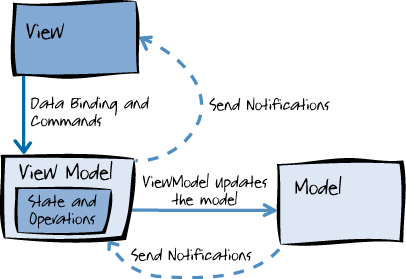
\includegraphics[scale=0.5]{Contenuto/Immagini/MVVM.png}
    \caption{Schema MVVM}
\end{figure}

In questo modo si ha una netta separazione tra chi salva ed elabora i dati (il Model) e chi li mostra (la View), mentre il View-Model funge da tramite tra le due parti. 
In accordo con il proponente, per realizzare la parte Frontend della WebApp, abbiamo scelto di utilizzare la libreria JavaScript React, per la quale viene fornita un'integrazione del meccanismo degli observer tramite la libreria \textit{MobX} (che abbiamo deciso di adottare per alcune componenti del nostro progetto).

In particolar modo, abbiamo implementato gli observer in alcune parti della:
\begin{itemize}
\item View, perché attende di aggiornarsi quando l’utente interagisce con la WebApp (p.es. sfruttiamo gli observer quanto l'utente effettua una ricerca o clicca su dei bottoni, operazioni tramite le quali l'utente si aspetta di ricevere qualcosa),
\item View-Model, perché questa parte rimane in attesa di ricevere una promise da parte del Model in merito alla “bontà” dell’operazione richiesta (nel caso l’operazione abbia esito positivo, vengono ritornati i dati da renderizzare nella View, altrimenti verrà ritornato un errore).
\end{itemize}